The scope of the calibration consortium includes a laser ionization system, a \phel laser system, a \dlong{lbls}, and a \dlong{pns} system. In addition, the consortium is evaluating a \dlong{rsds}. The calibration consortium is responsible for design through commissioning in the \dword{dpmod} for these calibration devices and their associated feedthroughs. Validating the designs of calibration systems at \dword{protodune2} (and other experiments as relevant) is also included under the scope of the consortium. Figure~\ref{fig:calib-scope_chart_V2} shows the subsystems included under the calibration consortium. 

Chapters 2, 3, 5, and 6 of Volume~\volnumberdp~(\voltitledp) of this \dword{tdr} describe other hardware essential for calibration such as \dword{crp} charge injection pulsing systems, \dword{hv} monitoring devices, \dword{pds} stability monitoring devices, and cryogenic instrumentation and detector monitoring devices, respectively. The scope of these systems is described by their respective consortia, and the calibration consortium has substantial interfaces with these consortia. 

The use of other calibration sources such as external measurements and existing sources of particles (e.g., muons, pions) is discussed in the calibration section of \dword{tdr} \physchtools. 

%The calibration task force (CTF) is 
We are pursuing the effects of calibration on physics and related studies. %, and the consortium works closely with the task force to make physics connections. 
Calibrations also require simulations (e.g., \efield) to identify desirable locations for calibration devices in the cryostat, away from regions of high \efield, so that their presence does not induce large field distortions. 
The design of the calibration systems and understanding the related physics requires coordination with other consortia and groups. This is discussed in Section~\ref{sec:dp-calib-intfc}.

\begin{dunefigure}[Calibration consortium subsystem chart]{fig:calib-scope_chart_V2}
{Calibration consortium subsystem chart. CTF stands for Calibration Task Force.}
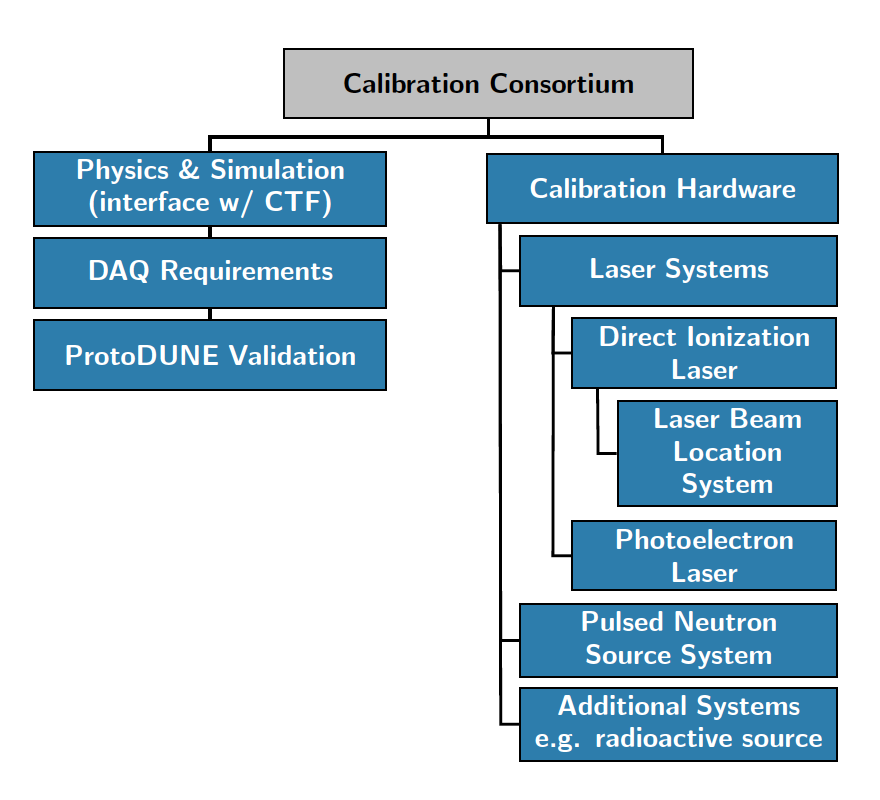
\includegraphics[height=4.0in]{graphics/calib-scope_chart_v3.png}
\end{dunefigure}
